\section{Anotações importantes da observação}

\subsection{Os primeiros vídeos}

O primeiro vídeo data de 09/MAI/2014, link \url{https://www.youtube.com/watch?v=8xyller_i5w}, ela com 12 anos ensinando a fazer caixas de doces decoradas, como denuncia a tag \#DIY\footnote{acrônimo de Do it Yourself, faça você mesmo} de Faça Você Mesmo. O vídeo é curto e demonstra que a menina possui desenvoltura e a mesma não se intimida pela câmera. A desenvoltura com que a mesma faz a caixa de doce sugere que ela já lida com trabalhos manuais com muita frequência.

Seguem-se outros vídeos com mesma temática de faça você mesmo, além de experimentação de guloseimas. Num deles faz um react\footnote{react é o termo usados pelos youtubers para reagir a algum fato pela primeira vez} de um unboxing de guloseimas comprados no bairro oriental da Liberdade em SP (\url{https://www.youtube.com/watch?v=qrBjcxeDKJE}). Ela dedica vários vídeos de doces orientais, incluindo os gravados com a mãe.

Nítido notar que a Zabetta é uma menina no final da puberdade, com feições infantis encontrados em qualquer menina da sua idade.

Ela mostra que já tem um time de coração, o Palmeiras, o que demonstra no vídeo \url{https://www.youtube.com/watch?v=W_LVN3bIKqo}, pena que não tem bastidores do pós-jogo para verificar as reações.

Durante um bom tempo ela se dedicou a vídeos de faça você mesma, muito inspirado nos trabalhos da mãe, Ane Macarini, que se considera Cake Design (Designer de Bolos). Inclusive fica evidente que a mãe incentiva e participa do conteúdo a ser produzido.

Como toda menina, ela sonha em ser atriz, inclusive fez teste de elenco com decoreba de texto no SBT\footnote{SBT - Sistema Brasileiro de Televisão} como demonstrado no vídeo \url{https://www.youtube.com/watch?v=iAzd_bcn_3c}. O vídeo é um grande registro de tietagem tanto dela como o da mãe. A relação com a mãe é de muita proximidade.

Interessante reparar que existe aprovação e controle da mãe sobre o conteúdo colocado no YouTube, o que seria normal da idade. Como a série de vídeos com o tema Halloween.

No vídeo \url{https://www.youtube.com/watch?v=f-FUL9s_0cU} foi um compilado de perguntas e respostas, onde é evidenciado que o pet da casa, uma cachorra chamada Bella. É revelado que Zabetta é um nome de origem italiana que possui tradição na família, o que reforça que existem laços e tradições fortes. A Zabetta já fez algumas figurações, o que responde sobre a desenvoltura em frente as câmeras.

No aniversário de 13 anos, ela demonstrou seus presentes no vídeo \url{https://www.youtube.com/watch?v=nCskv33ok08} o fato curioso é ela ter ganho um cartão de crédito do tipo mesada, indicando preocupação dos pais com a educação financeira ou controle do que é gasto pela filha. O engajamento do colégio (Objetivo) com seus alunos foi mencionado na festa surpresa preparada pela mãe e as coordenadoras. A fala é desenvolta mas compatível do que se espera de vocabulário e articulação de uma criança de 13 anos. Fora uma comemoração em família no Outback no vídeo \url{https://www.youtube.com/watch?v=Fsuw8c0nYP0}.

\begin{figure}
    \centering
    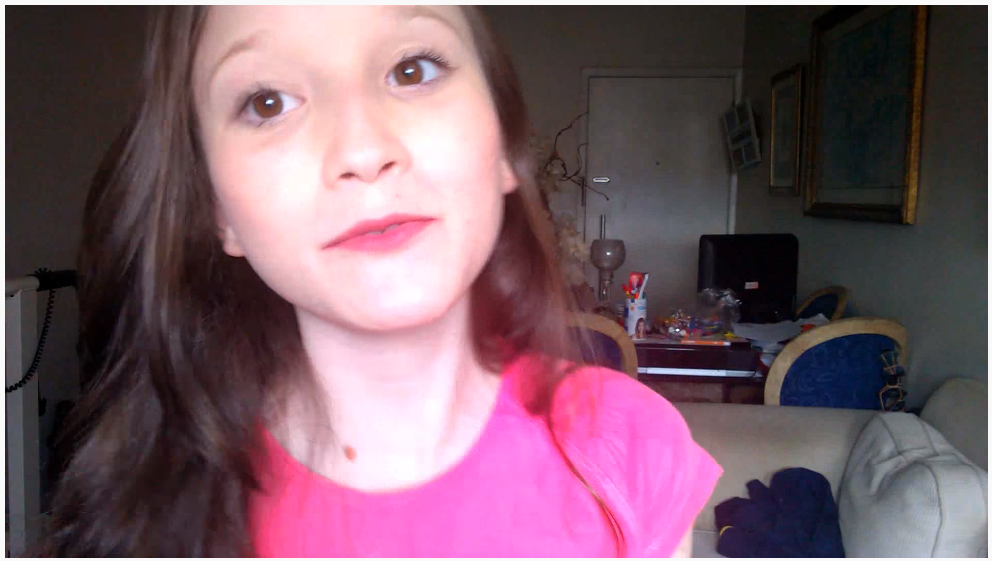
\includegraphics[width=0.7\linewidth]{fig/Zabetta-13-anos}
    \caption{vb}
    \label{fig:zabetta-13-anos}
\end{figure}


No vídeo \url{https://www.youtube.com/watch?v=QDMu3dTOoVI} ela brinca num desafio com cereja e chantily vemos que ela é a caçula de outros 3 irmãos. Aparentemente eles são muito amorosos um com outro.

No vídeo \url{https://www.youtube.com/watch?v=z0VjIP5AUAU} ela se permite mostrar alguns erros de gravação, mostrando um pouco dela como ela realmente é. Nesse vídeo mostra a interação com produtos que ela ganhou de aniversário. Fácil notar que tirando o HD e o PowerBank indutivo, todos os demais produtos são do universo feminino, maquiagem e beleza.



Em \url{https://www.youtube.com/watch?v=cH0fpW70ujY} ela faz algo muito típico de meninas no YouTube na idade dela: tutorial de maquilagem e como se vestir. É o jantar do ano novo de 2015, a falta do pai sugere que ela é filha de pais separados.

Vemos um exemplo de interação social no vídeo \url{https://www.youtube.com/watch?v=m46LF9b9NqU} referente a entrega de um prêmio para assinantes do canal. Tudo muito improvisado e rola uma certa timidez. Talvez fruto de não se preparar muito bem para a ocasião.

Um vídeo bem comum entre as meninas adolescentes youtubers é o react do seu material escolar no início do ano, como nesse vídeo referente ao começo do ano de 2015 em \url{https://www.youtube.com/watch?v=nXG0OKnmHpo}. O objetivo é claro, lançar tendências e mostrar seu stylelife\footnote{stylelife é estilo de vida.}. Curioso que o nível de exigência, talvez pela idade seja pouco.

Em \url{https://www.youtube.com/watch?v=N409jTfwMCg} ela se demonstra mais solta talvez por que achou engraçada a experiencia de andar horas seguidas no carro e precisou criar formas criativas e fofas de se livrar do tédio.

No vídeo \url{https://www.youtube.com/watch?v=wTd6gUh6BxI} comemoram 2 mil inscritos, o canal hoje tem 2,73 milhões.

No episódio \textbf{Meu celular foi destruído} \url{https://www.youtube.com/watch?v=-WGYaDwg0Fg} temos demonstrações de emoções como choro emocionado pelo celular novo que a mãe comprou e sua indignação pela quebra do celular. É nítido a frustração que ela não consegue falar o que aconteceu, provavelmente algo bobo que ela se envergonha. Importante verificar que existe uma consciência da mãe de que os jovens não podem ficar sem celular. A impressão que o aparelho é um "módulo de proteção" dos pais para com os filhos, já que permite comunicação instantânea com o rebento a qualquer hora. Pais mais neuróticos colocam rastreamento.

No episódio \textbf{\#Zabetta na cozinha - Bolo de Cenoura} \url{https://www.youtube.com/watch?v=pRk6TOCBrkY} ela mostra amigas de colégio, provavelmente do 9 ano do ensino fundamental. Ao contrário da protagonista as demais pessoas são muito tímidas, o que demonstra o contraste do preparo que a mesma faz para estar diante das câmeras.

No episódio Fale qualquer coisa \url{https://www.youtube.com/watch?v=G_XT9Ghtnpo} demonstra brincadeiras comuns entre youtubers jovens em busca de views por meio de humor pastelão. A interação com a mãe é engraçadíssimo.

Em \href{https://www.youtube.com/watch?v=WuJ_XpMSIws}{\textbf{\#VEDA - Tirando Dúvidas (MODELO,AGENCIA) (day 15)}} \url{https://www.youtube.com/watch?v=WuJ_XpMSIws} a mãe e a protagonista tiram dúvidas sobre a carreira de modelo, agenciamento. Existe uma nítida preocupação com os estudos e o futuro da menina. Tudo de forma bem transparente entre mãe e filha o que denuncia o cuidado da mãe com a filha caçula. Interessante a lista de documentos para permitir o trabalho da menor de idade em produtoras para gravação de um comercial.

A quantidade de inscritos chegou em 10 mil comemorados no vídeo \href{https://www.youtube.com/watch?v=KrqZuiVizzg}{\textbf{10.000 Inscritos \#VEDA (day 23 )}}. \url{https://www.youtube.com/watch?v=KrqZuiVizzg} onde a protagonista mostra depoimentos de fãs do próprio colégio dela. Interessante os depoimentos que mostram alguma hiperatividade e atitudes típicas de alunos do final do ensino fundamental. Detalhe do aluno que diz que não é gay embora pareça. Fiquei me perguntando dos esteriótipos e o bullying que ele vem sofrendo. Confesso que senti uma ponta de inveja e saudade da minha oitava série em 1988. A quantidade de amigos demonstrados foi muito alta. A sensação de pertencimento de um grupo é muito forte nesse vídeo. A comunidade de inscrito gira entre 10 e 17 anos em média pela aparência. A internet e as redes sociais diminuíram muito a distância entre ídolos e seus fãs, além de que não é mais necessário ter uma participação na TV para alavancar a carreira, sendo a divulgação boca a boca muito poderosa nesse meio.

O vídeo \href{https://www.youtube.com/watch?v=kRku3MWoG8A}{\textbf{Especial dia das mães}} \url{https://www.youtube.com/watch?v=kRku3MWoG8A} corrobora com a observação acima em que ela demonstra a emoção pela data especial.

No vídeo \href{https://www.youtube.com/watch?v=VRcU2faTZc4}{OBJETIVO - Vlog na Escola} \url{https://www.youtube.com/watch?v=VRcU2faTZc4} ela demonstra algumas cenas da escola em que ela estuda. Fascinante a vergonha diante da classe, a posição de destaque ou liderança perante a classe, mesmo que seja um amigo oculta.

Em \href{https://www.youtube.com/watch?v=KBkS6t55zEM}{MINHA MÃE FICOU MUITO BRAVA } \url{https://www.youtube.com/watch?v=KBkS6t55zEM} temos a oportunidade de ver bastidores da mãe editando os vídeos para o canal e uma trolagem da protagonista com a mãe usando um cabelo. Hilário e agonizante.

Nos episódios \href{https://www.youtube.com/watch?v=ezL9_lYwRWs}{Minha Rotina 2015 realidade na escola - TRAILER} \url{https://www.youtube.com/watch?v=ezL9_lYwRWs} e \href{https://www.youtube.com/watch?v=4cjxIiDx9yk}{\textbf{Vlog - Minha Rotina na Escola 2015}} \url{https://www.youtube.com/watch?v=4cjxIiDx9yk} temos oportunidade de ver algumas atividades que o colégio da protagonista desempenha com seus alunos. Experimentos de química, dança, entre outros. Além de encontros com fãs e amigas treslocadas no vídeo.

O canal comemora 1 ano com 30 mil inscrito com uma live \href{https://www.youtube.com/watch?v=Jp_d0ItrVS8}{\textbf{LIVE aovivo Comemoração: 30k Inscritos e 1 Ano de Canal}} \url{https://www.youtube.com/watch?v=Jp_d0ItrVS8}. A mãe comentou que ela deleta comentários de haters para não magoar a protagonista.

No vídeo \href{https://www.youtube.com/watch?v=JMyCKVb5rOA}{Vlog: Encontrinho Youtubers Mirins SP} \url{https://www.youtube.com/watch?v=JMyCKVb5rOA} foi num encontro de youtubers mirins e seus fãs. Nítido ver o progresso da protagonista, a desenvoltura, etc...

\begin{figure}[h!]
    \centering
    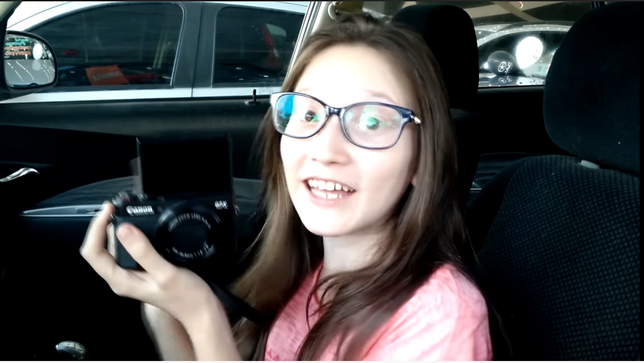
\includegraphics[width=0.7\linewidth]{fig/Zabetta-15-anos}
    \caption{Zabette 15 anos}
    \label{fig:zabetta-15-anos}
\end{figure}


\subsection{Vídeos mais relevantes}

Visando otimizar o estudo, vamos acelerar e só coletar vídeos mais relevantes.

No episódio \href{https://www.youtube.com/watch?v=1Xa5F_aFzVY}{Vlog - 1º ano do Ensino Médio : Primeiro dia de aula! FEV. 2016} \url{https://www.youtube.com/watch?v=1Xa5F_aFzVY} mostra os bastidores do primeiro dia de aula no ensino médio. Não foi um dia de integração como em outras instituições. Aparentemente é uma sala de colegas que passaram junto com a protagonista.

Em março de 2016 ela mostrou sua \href{https://www.youtube.com/watch?v=-t4_4_55LbI}{TOP 10 - MINHA PLAYLIST | 10 MÚSICAS FAVORITAS!} \url{https://www.youtube.com/watch?v=-t4_4_55LbI} o que demonstra uma predileção por sucessos pop e funk muito tocadas no próprio youtube e no Spotify.

Como todo adolescente em 2016 a protagonista entrou no fenômeno cultural do Pokemon Go. Em \href{https://www.youtube.com/watch?v=t6SLGg9ul1g}{FUI CAÇAR POKÉMON NA ESCOLA! - Pokémon Go} \url{https://www.youtube.com/watch?v=t6SLGg9ul1g} ela demonstra a febre e como dominou o cenário no começo desse ano. O vídeo demonstra os corredores do colégio e várias pessoas aderindo ao jogo.

Após algumas esquetes com a mãe, surge um vídeo com título chamativo \href{https://www.youtube.com/watch?v=nGa7vxsb15I}{Vlog - COMO FOI MINHA PRIMEIRA VEZ} \url{https://www.youtube.com/watch?v=nGa7vxsb15I} que fala do seu primeiro voo de avião. Logicamente surge uma curiosidade natural que ela pode falar de sua sexualidade, mas em face ao conteúdo anterior só se surpreenderá quem nunca viu seu canal. As caras e bocas de medo da decolagem são as melhores cenas.

Um vídeo que demonstra muito bem o choque de gerações é o episódio \href{https://www.youtube.com/watch?v=saR5sjRjiPc}{MINHA MÃE REAGINDO AOS PROIBIDÃO! \#2}
 \url{https://www.youtube.com/watch?v=saR5sjRjiPc}, provavelmente o primeiro foi retirado por algum motivo. Foram várias músicas de funk com várias palavras de baixo calão e sexualizadas. Nítido notar que existe muito diálogo sobre qualquer assunto, incluindo sobre esse tema. Outro vídeo da mesma época \href{https://www.youtube.com/watch?v=zy0ejd8z8Sg}{MÃES REAGINDO AOS PESADÕES !! \#3} \url{https://www.youtube.com/watch?v=zy0ejd8z8Sg} temos reação com mais um jovem da mesma idade e sua mãe.

Em \href{https://www.youtube.com/watch?v=C8tlm_j_Xbg}{\textbf{MEU MATERIAL ESCOLAR 2017}} \url{https://www.youtube.com/watch?v=C8tlm_j_Xbg} é nítido o crescimento e a desenvoltura que estão mais maduras.

No episódio \href{https://www.youtube.com/watch?v=XKOwncyuNu0}{NÃO ACREDITO FUI EXPULSA DO SHOPPING !!} \url{https://www.youtube.com/watch?v=XKOwncyuNu0} ela experimenta da forma mais maluca a explosão de membros de seu canal enchendo o saguão de um shopping. Muita gente foi lá para vela. Para segurança foi solicitado a dispersão. Nítido a frustração da protagonista.

No primeiro dia de aula (\url{https://www.youtube.com/watch?v=B18Yur2bvkI}) mostra mais um dia normal, nota-se que o colégio não adota um uniforme. Ela demonstra que o canal tem quase 800 mil seguidores. no episódio \url{https://www.youtube.com/watch?v=tFvm_aEzEe0} referente à primeira semana de aula, onde temos demonstrações de mongolice explicita. Saudade dessa bagunça no meu tempo. Fica latente o amadurecimento da protagonista.

Em \href{https://www.youtube.com/watch?v=3VdpUWt3xns}{\textbf{PERGUNTAS DE FÃS}} \url{https://www.youtube.com/watch?v=3VdpUWt3xns} além de trolagens e desafios sem sentido ou noção Vemos a evolução da cachorra dela. Mais um thumbnail\footnote{imagem da capa do vídeo} pescando a imaginação dos expectadores com seu signo.

No \href{https://www.youtube.com/watch?v=s1XCblDI9K4}{\textbf{DESABAFO}} \url{https://www.youtube.com/watch?v=s1XCblDI9K4} a mãe fala dos comentários maldosos de seu canal mostrando a prioridade da Zabetta, que deve ser os estudos. É de fato um desabafo e um pedido a todos tenham empatia. O sembrante da protagonista fica carregada, demonstrando indignação. Clima mais pesado.

Mais um vídeo de primeiro dia de aula (\url{https://www.youtube.com/watch?v=r6OCOTCHjXY}), recomeço em agosto, mais um festival de traquinagens nos intervalos entre aulas e recreio. A câmera deve ligar o modo mongoloide de todos.

Outro vídeo interessante é \href{https://www.youtube.com/watch?v=NnmVopUTL4c}{\textbf{MÁSCARA PRETA PARA REMOVER CRAVOS - SERÁ??}} \url{https://www.youtube.com/watch?v=NnmVopUTL4c} traz receitas para remover cravos. bizarro. Claro interesse com sua estética.

Temos mais uma sessão de perguntas e respostas, \href{https://www.youtube.com/watch?v=AQd3wlIH-QI}{\textbf{QUE MANCHA É ESSA ???}} (\url{https://www.youtube.com/watch?v=AQd3wlIH-QI}). Trolando a amiga sobre namoro. Interessante que o assunto namoro de colegas é muito delicado. A insegurança do tema é latente. Conselhos amorosos devem ser assunto recorrente nas rodas de jovens. Perda de amizades, micos, vergonha alheia. Os medos, ciúmes, a autocobrança para não errar. Sobre marcas no próprio corpo confundindo com chupão. Muita insegurança.

Fato curioso, ela comemorou 16 anos e não 15 anos, como mostrado em \href{https://www.youtube.com/watch?v=VzXQh5oLdPM}{Minha festa de 16 anos} \url{https://www.youtube.com/watch?v=VzXQh5oLdPM}. Acredito que foi a festa dos sonhos dela. Uma postura mais madura, não de uma criancinha.

Em \href{https://www.youtube.com/watch?v=L-4JjjRVzHo}{\textbf{DESAFIOS NAS RUAS DE SP}} \url{https://www.youtube.com/watch?v=L-4JjjRVzHo} que é mais uma sessão de perguntas e respostas, mostram mais inseguranças para não errar com coisas banais como não reconhecer direito uma amiga que queria cumprimentar e ficou com vergonha e sobre problemas com notas. Vale a menção que ela tenta responder as perguntas com o máximo de sinceridade possível. Uma pergunta filosófica do tipo prefere uma borracha para apagar o passado ou um lápis para escrever o futuro ela mencionar preferir o lápis.

\begin{figure}[h!]
    \centering
    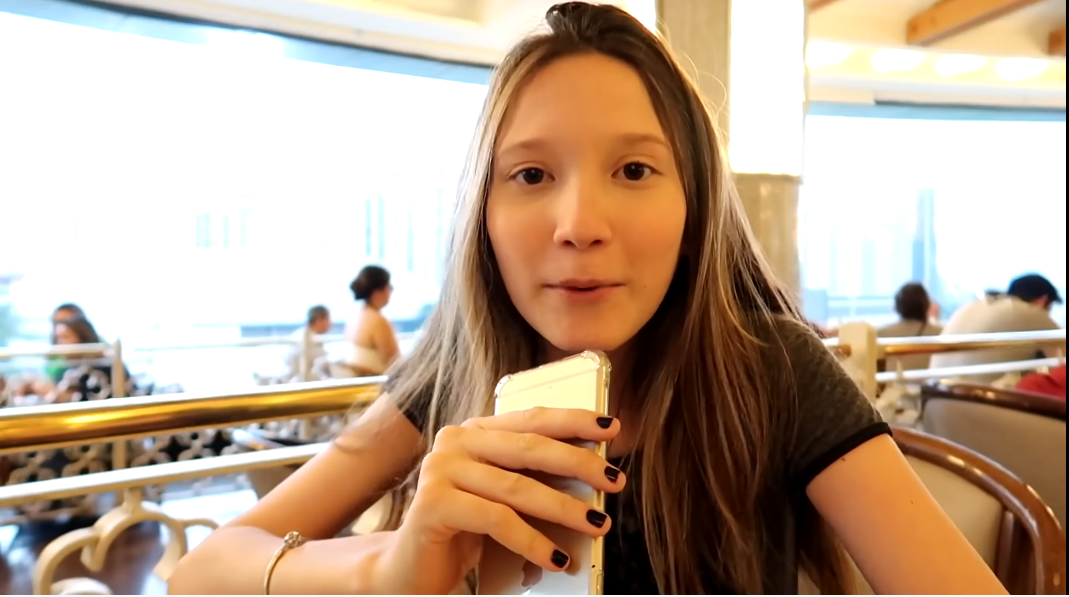
\includegraphics[width=0.7\linewidth]{fig/Zabetta-16-anos1}
    \caption{16 anos}
    \label{fig:zabetta-16-anos1}
\end{figure}




